\chapter{Deployment}
Il progetto sviluppato si compone di tre applicazioni:

\begin{itemize}
    \item Applicazione Client backend;
    \item Applicazione Simulator;
    \item Applicazione Hololens.
\end{itemize}

Le prime due sono rilasciate su GitHub, pertanto basterà recuperare l'ultima release dal nostro repository a questo \href{https://github.com/lucagiorgettismp/AzureHealthcareDigitalTwins/releases}{\textit{link}}.
Allegati alla release si trovano i file .zip contenenti gli eseguibili di Client e Simulator.

\section{Client backend}
L'applicazione client di backend permette di visualizzare le schede paziente precedentemente create e la creazione di nuovi pazienti. Per poter utilizzare il sistema progettato, è necessario che almeno un paziente sia stato creato prima di avviare il simulatore, in quanto al momento della creazione della scheda paziente viene creato anche il device IoTHub per il relativo monitor parametri vitali.

\begin{figure}[H]
    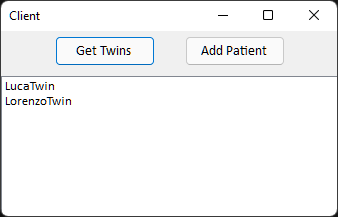
\includegraphics[width=6cm]{client_screen.png}
    \centering
    \caption{\label{pic:client-deployment}Schermata principale del client.}
\end{figure}

\section{Simulatore backend}
Questa applicazione permette di simulare l'asset fisico, pertanto è necessario che venga avviata per emettere dati sul monitor parametri vitali del paziente. \newline \newline All'apertura, viene recuperata la lista dei devices presenti, e una volta selezionato quello desiderato (eventualmente creato tramite il Client al paragrafo precedente), è possibile configurare range dei valori, unità di misura e soglie di allarme. Diversamente, il simulatore viene avviato con i valori di default.
Con il device selezionato, è possibile avviare il monitor parametri vitali che ad ogni iterazione genererà nuovi valori che verranno notificati al digital twin.\\
\newline Se il simulatore è spento, non viene aggiornato il digital twin, pertanto non viene inviato nessun messaggio su SignalR.

\begin{figure}[H]
    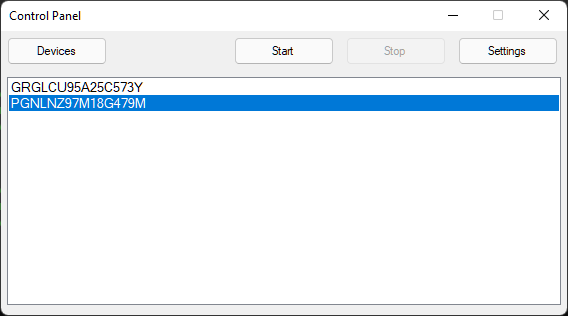
\includegraphics[width=10cm]{simulator_screen.png}
    \centering
    \caption{\label{pic:simulator-deployment}Schermata di selezione device.}
\end{figure}

\section{Applicazione Hololens}
Non essendo rilasciata su Microsoft Store, la nostra applicazione deve essere prima compilata, ed in seguito rilasciata sul device Hololens.

Durante lo sviluppo abbiamo utilizzato Unity v2020.3.4f1 e Visual Studio 2019 v16.11.11.

\subsection{Import di Mixed Reality Toolkit}
Prima di aprire il progetto, è necessario importare le componenti del Mixed Reality Toolkit.
\begin{enumerate}
    \item Avviare il Mixed Reality Toolkit (MixedRealityFeatureTool) scaricato
precedentemente.
    \item Fare clic sull’icona dell’ingranaggio.
    \item  Nella sezione Feature Settings, attivare “Show preview releases” e cliccare su OK.
    \item Fare clic su Start.
    \item Impostare il percorso del progetto Unity creato precedentemente e fare clic su “Discover Features”.
    \item Nella sezione “Mixed Reality Toolkit” selezionare “Mixed Reality Toolkit foundation”
    \item Nella sezione “Platform Support” selezionare “Mixed Reality OpenXR Plugin”.
    \item Cliccare su ”Get Features”.
    \item Cliccare su “Validate”, poi su OK e infine su Import.
    \item Cliccare su “Approve” e poi su “Exit”, a questo punto i componenti dovrebbero essere stati importati in Unity correttamente.
\end{enumerate}

\subsection{Configurazione di Mixed Reality Toolkit}
Aprendo il progetto su Unity dovrebbe comparire la finestra “MRTK Project Configurator”. In caso contrario, la si può aprire da menù \\ 
Mixed Reality > Toolkit > Utilities > Configure Project for MRTK.
\begin{enumerate}
    \item Controllare che tutte le opzioni siano spuntate e cliccare su “Apply”, a questo punto Unity dovrebbe riavviarsi.
    \item Selezionare Edit > Project Settings.
    \item Selezionare XR Plug-in Management > Install XR Plug-in Management.
    \item In Universal Windows Platform attivare “ XR Plug-in Management > Install XR Plug-in Management”, “OpenXR” e “Microsoft HoloLens feature set”.
    \item Se sono presenti dei warning cliccare sul punto esclamativo e poi su “Fix All”, dovrebbero scomparire.
\end{enumerate}

\subsection{NuGet}
E' necessario installare NuGet in Unity e scaricare i pacchetti utilizzati dal nostro progetto:

\begin{enumerate}
    \item Installare NuGet il wiki presente al seguente link: \url{https://github.com/GlitchEnzo/NuGetForUnity}.
    \item Riavviare Unity.
    \item Scaricare i pacchetti utilizzati tramite menu NuGet > Restore Packages.
\end{enumerate}

\subsection{Build e Deploy}

\begin{enumerate}
    \item In Unity selezionare File > Build Settings.
    \item Cliccare su Add Open Scenes per aggiungere le scene.
    \item Configuare la build come mosttrato in figura \ref{pic:build-settings}.
    
    \begin{figure}[H]
        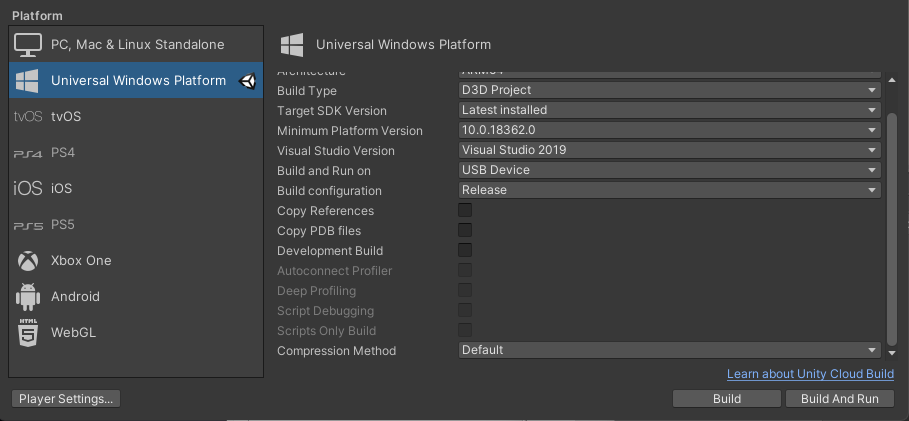
\includegraphics[width=12cm]{hololens_build_settings.png}
        \centering
        \caption{\label{pic:build-settings}Build settings.}
    \end{figure}
    
    \item Cliccare su “Build” e selezionare la cartella delle build (solitamente “Builds”, nella directory del progetto Unity)
    \item Dopo aver compilato dovrebbe aprire una nuova finestra del gestore dei file, entrare nella cartella delle build e avviare il progetto di Visual Studio.
    \item In Visual Studio selezionare “Release”, architettura: “ARM64”, target: “Device” 
    \item Collegare Hololens 2 al PC (Usare le porte USB della scheda madre se possibile)
    \item Quando si fa il deploy da un nuovo PC per la prima volta bisogna fare il pairing dei device:
    \item Su Visual Studio avviare il deploy da Build > Deploy solution, verrà richiesto un PIN.
    \item Su Hololens andare in Settings > For Developers e cliccare su “Pair”, comparirà un PIN, inserirlo in Visual Studio.
    \item A questo punto si può accedere all’app installata direttamente dal menu delle applicazioni di Hololens 2.
\end{enumerate}

\subsection{Creazione QR code}
    E' possibile utilizzare uno dei QR code presenti in all'interno della release su GitHub, oppure generarne uno custom; in questo caso:
    \begin{enumerate}
        \item Andare all'url \url{https://www.qrcode-monkey.com/en/#text}.
        \item Inserire una stringa di tipo Json fatta come segue:
        \begin{lstlisting}[language=json, firstnumber=1]
{"deviceId": "CODICE_FISCALE_DEL_PAZIENTE"}
        \end{lstlisting}
        \item Generare e scaricare il QR code appena creato.
    \end{enumerate}

Una volta avviata l'applicazione su Hololens, inquadrare il QR code. \\
\newline Quando viene rilevato l'identificativo del paziente, verranno caricate le informazioni sul paziente, il menù di selezione delle schermate e la schermata precedentemente selezionata (o di default la schermata Home se si tratta della prima apertura).